\section{Vessel Manoeuvring Models} \label{sec:VMM}
\label{\detokenize{02.01_VMMs:vessel-manoeuvring-models}}\label{\detokenize{02.01_VMMs:vmm}}\label{\detokenize{02.01_VMMs::doc}}
\sphinxAtStartPar
Ship manoeuvring is a simplified case of seakeeping. The encountering waves have been removed, assuming calm water conditions. This simplification allows the ship dynamics to be expressed with only four degrees of freedom: surge, sway, roll, and yaw, where the roll is often excluded. Surge, sway, and yaw have very low frequencies during manoeuvres, so added masses and other hydrodynamic derivatives can be assumed as constants  \cite{fossen_handbook_2021}. Three Vessel Manoeuvring Models (VMMs) are used in this thesis: Linear (LVMM) \cite{matusiak_dynamics_2017}, Abkowitz (AVMM), \cite{abkowitz_ship_1964} and Modified Abkowitz (MAVMM), which is proposed in this thesis.
\hyperref[\detokenize{02.01_VMMs:coordinate-system}]{Fig.\@ \ref{\detokenize{02.01_VMMs:coordinate-system}}} shows the reference frames used in the VMMs where \(x_0\) and \(y_0\) and heading \(\Psi\) are the global position and orientation of a ship fix reference frame \(O(x,y,z)\) (or rather \(O(x,y)\) when heave is exluded) with origin at midship. \(u\), \(v\), \(r\), \(X\), \(Y\) and \(N\) are velocities and forces in the ship fix reference frame.



\begin{figure}[h]
    \centering
    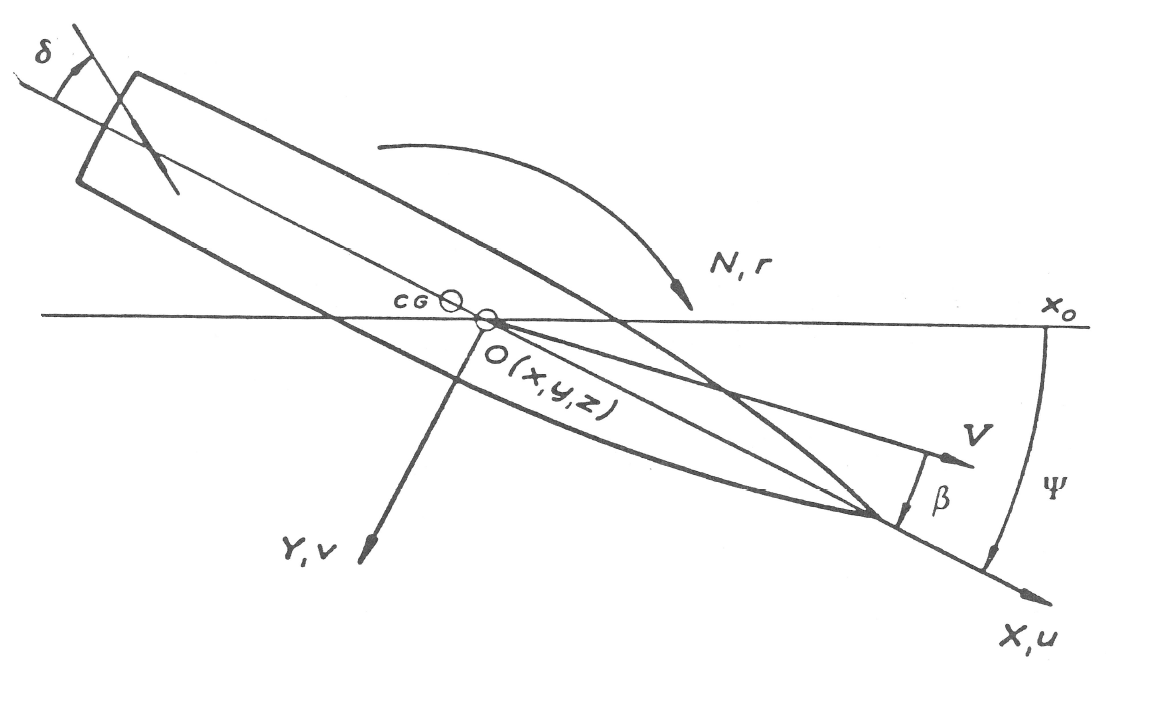
\includegraphics[width=\textwidth]{kappa/images/coordinate_system.PNG}
    \caption{Coordinate system}
    \label{\detokenize{02.01_VMMs:coordinate-system}}
\end{figure}

\sphinxAtStartPar
The acceleration can be solved from the manoeuvring equation (\autoref{equation:02.01_VMMs:eqqsystem}) \cite{fossen_handbook_2021} as seen in \autoref{equation:02.01_VMMs:eqacc},
\begin{equation}\label{equation:02.01_VMMs:eqqsystem}
\begin{split}\displaystyle \left[\begin{matrix}- X_{\dot{u}} + m & 0 & 0\\0 & - Y_{\dot{v}} + m & - Y_{\dot{r}} + m x_{G}\\0 & - N_{\dot{v}} + m x_{G} & I_{z} - N_{\dot{r}}\end{matrix}\right] \left[\begin{matrix}\dot{u}\\\dot{v}\\\dot{r}\end{matrix}\right] = \left[\begin{matrix}m r^{2} x_{G} + m r v + \operatorname{X_{D}}{\left(u,v,r,\delta,thrust \right)}\\- m r u + \operatorname{Y_{D}}{\left(u,v,r,\delta,thrust \right)}\\- m r u x_{G} + \operatorname{N_{D}}{\left(u,v,r,\delta,thrust \right)}\end{matrix}\right]\end{split}
\end{equation}\begin{equation}\label{equation:02.01_VMMs:eqacc}
\begin{split}\displaystyle \dot{\nu} = \left[\begin{matrix}\dot{u}\\\dot{v}\\\dot{r}\end{matrix}\right] = \left[\begin{matrix}\frac{1}{- X_{\dot{u}} + m} & 0 & 0\\0 & - \frac{- I_{z} + N_{\dot{r}}}{S} & - \frac{- Y_{\dot{r}} + m x_{G}}{S}\\0 & - \frac{- N_{\dot{v}} + m x_{G}}{S} & - \frac{Y_{\dot{v}} - m}{S}\end{matrix}\right] \left[\begin{matrix}m r^{2} x_{G} + m r v + \operatorname{X_{D}}{\left(u,v,r,\delta,thrust \right)}\\- m r u + \operatorname{Y_{D}}{\left(u,v,r,\delta,thrust \right)}\\- m r u x_{G} + \operatorname{N_{D}}{\left(u,v,r,\delta,thrust \right)}\end{matrix}\right]\end{split}
\end{equation}
\sphinxAtStartPar
where \(S\) is a helper variable:
\begin{equation}\label{equation:02.01_VMMs:eq_S}
\begin{split}\displaystyle S = - I_{z} Y_{\dot{v}} + I_{z} m + N_{\dot{r}} Y_{\dot{v}} - N_{\dot{r}} m - N_{\dot{v}} Y_{\dot{r}} + N_{\dot{v}} m x_{G} + Y_{\dot{r}} m x_{G} - m^{2} x_{G}^{2}\end{split}
\end{equation}
\sphinxAtStartPar
A state space model for manoeuvring can now be defined with six states:
\begin{equation}\label{equation:02.01_VMMs:eq_x}
\begin{split}\displaystyle \mathbf{x} = \left[\begin{matrix}x_{0}\\y_{0}\\\Psi\\u\\v\\r\end{matrix}\right]\end{split}
\end{equation}
\sphinxAtStartPar
The time derivative of this state \(\dot{\mathbf{x}}\) can be defined by a state transition \(f(\mathbf{x},\mathbf{c})\) using geometrical relations
how global coordinates \(x_0\), \(y_0\) and \(\Psi\) depend on \(u\), \(v\), and \(r\) viz.,
\begin{equation}\label{equation:02.01_VMMs:eqf}
\begin{split}\displaystyle \dot{\mathbf{x}} = f(\mathbf{x},\mathbf{c}) + \mathbf{w}
                                          = \left[\begin{matrix}\dot{x_0}\\ \dot{y_0} \\ \dot{\Psi} \\\dot{u}\\\dot{v}\\\dot{r}\end{matrix}\right] + \mathbf{w}
                                          = \left[\begin{matrix}u \cos{\left(\Psi \right)} - v \sin{\left(\Psi \right)}\\u \sin{\left(\Psi \right)} + v \cos{\left(\Psi \right)}\\r\\\dot{u}\\\dot{v}\\\dot{r}\end{matrix}\right] + \mathbf{w}\end{split}
\end{equation}
\sphinxAtStartPar
where \(\mathbf{c}\) is control inputs (rudder angle \(\delta\) and thrust); the last three derivatives: \(\dot{u}\), \(\dot{v}\), \(\dot{r}\) are calculated with \autoref{equation:02.01_VMMs:eqacc}.
\(\mathbf{w}\) is the process noise, i.e., the difference between the predicted state by the VMM and the true
state of the system. \(\mathbf{w}\) is unknown when the VMM is used for manoeuvre predictions and therefore normally
assumed to be zero, but it is an important factor when the VMM is used in the EKF, see Section \ref{sec:datacleaning}.
The manoeuvring simulation can now be conducted by numerical integration of \autoref{equation:02.01_VMMs:eqf}. The main difference between the VMM:s lies in how the hydrodynamic functions \(X_D(u,v,r,\delta,thrust)\), \(Y_D(u,v,r,\delta,thrust)\), \(N_D(u,v,r,\delta,thrust)\) are defined. These expressions are denoted below for the various VMMs: LVMM, AVMM and MAVMM.

\sphinxAtStartPar
LVMM (Linear Vessel Manoeuvring Model) \cite{matusiak_dynamics_2017}:
\begin{equation}\label{equation:02.01_VMMs:eqxlinear}
\begin{split}\begin{split}
\operatorname{X_{D}'}{\left(u',v',r',\delta,thrust' \right)} = & X_{\delta} \delta + X_{r} r' + X_{u} u' + X_{v} v' 
\end{split}\end{split}
\end{equation}\begin{equation}\label{equation:02.01_VMMs:eqylinear}
\begin{split}\begin{split}
\operatorname{Y_{D}'}{\left(u',v',r',\delta,thrust' \right)} = & Y_{\delta} \delta + Y_{r} r' + Y_{u} u' + Y_{v} v' 
\end{split}\end{split}
\end{equation}\begin{equation}\label{equation:02.01_VMMs:eqnlinear}
\begin{split}\begin{split}
\operatorname{N_{D}'}{\left(u',v',r',\delta,thrust' \right)} = & N_{\delta} \delta + N_{r} r' + N_{u} u' + N_{v} v' 
\end{split}\end{split}
\end{equation}
\sphinxAtStartPar
AVMM (Abkowitz Vessel Manoeuvring Model) \cite{abkowitz_ship_1964}:
\begin{equation}\label{equation:02.01_VMMs:eqxabkowitz}
\begin{split}
\operatorname{X_{D}'}{\left(u',v',r',\delta,thrust' \right)} = & X_{\delta\delta} \delta^{2} + X_{r\delta} \delta r' + X_{rr} r'^{2} + X_{T} thrust' + X_{u\delta\delta} \delta^{2} u' \\ 
& + X_{ur\delta} \delta r' u' + X_{urr} r'^{2} u' + X_{uuu} u'^{3} + X_{uu} u'^{2} \\ 
& + X_{uv\delta} \delta u' v' + X_{uvr} r' u' v' + X_{uvv} u' v'^{2} \\
& + X_{u} u' + X_{v\delta} \delta v' + X_{vr} r' v' + X_{vv} v'^{2} 
\end{split}
\end{equation}

\begin{equation}\label{equation:02.01_VMMs:eqyabkowitz}
\begin{split}\begin{split}
\operatorname{Y_{D}'}{\left(u',v',r',\delta,thrust' \right)} = & Y_{0uu} u'^{2} + Y_{0u} u' + Y_{0} + Y_{\delta\delta\delta} \delta^{3} + Y_{\delta} \delta + Y_{r\delta\delta} \delta^{2} r' + Y_{rr\delta} \delta r'^{2} + Y_{rrr} r'^{3} \\
& + Y_{r} r' + Y_{T\delta} \delta thrust' + Y_{T} thrust' + Y_{u\delta} \delta u' + Y_{ur} r' u' + Y_{uu\delta} \delta u'^{2} + Y_{uur} r' u'^{2} + Y_{uuv} u'^{2} v' \\
& + Y_{uv} u' v' + Y_{v\delta\delta} \delta^{2} v' + Y_{vr\delta} \delta r' v' + Y_{vrr} r'^{2} v' + Y_{vv\delta} \delta v'^{2} + Y_{vvr} r' v'^{2} + Y_{vvv} v'^{3} + Y_{v} v' 
\end{split}\end{split}
\end{equation}\begin{equation}\label{equation:02.01_VMMs:eqnabkowitz}
\begin{split}\begin{split}
\operatorname{N_{D}'}{\left(u',v',r',\delta,thrust' \right)} = & N_{0uu} u'^{2} + N_{0u} u' + N_{0} + N_{\delta\delta\delta} \delta^{3} + N_{\delta} \delta + N_{r\delta\delta} \delta^{2} r' + N_{rr\delta} \delta r'^{2} + N_{rrr} r'^{3} \\
& + N_{r} r' + N_{T\delta} \delta thrust' + N_{T} thrust' + N_{u\delta} \delta u' + N_{ur} r' u' + N_{uu\delta} \delta u'^{2} + N_{uur} r' u'^{2} + N_{uuv} u'^{2} v' \\
& + N_{uv} u' v' + N_{v\delta\delta} \delta^{2} v' + N_{vr\delta} \delta r' v' + N_{vrr} r'^{2} v' + N_{vv\delta} \delta v'^{2} + N_{vvr} r' v'^{2} + N_{vvv} v'^{3} + N_{v} v' 
\end{split}\end{split}
\end{equation}
\sphinxAtStartPar
MAVMM (Modified Abkowitz Vessel Manoeuvring Model, where only the most relevant coefficients in AVMM are included.)
\begin{equation}\label{equation:02.01_VMMs:eqxmartinssimple}
\begin{split}\begin{split}
\operatorname{X_{D}'}{\left(u',v',r',\delta,thrust' \right)} = & X_{\delta\delta} \delta^{2} + X_{rr} r'^{2} + X_{T} thrust' + X_{uu} u'^{2} + X_{u} u' + X_{vr} r' v' 
\end{split}\end{split}
\end{equation}\begin{equation}\label{equation:02.01_VMMs:eqymartinssimple}
\begin{split}\begin{split}
\operatorname{Y_{D}'}{\left(u',v',r',\delta,thrust' \right)} = & Y_{\delta} \delta + Y_{r} r' + Y_{T\delta} \delta thrust' + Y_{T} thrust' + Y_{ur} r' u' + Y_{u} u' + Y_{vv\delta} \delta v'^{2} + Y_{v} v' 
\end{split}\end{split}
\end{equation}\begin{equation}\label{equation:02.01_VMMs:eqnmartinssimple}
\begin{split}\begin{split}
\operatorname{N_{D}'}{\left(u',v',r',\delta,thrust' \right)} = & N_{\delta} \delta + N_{r} r' + N_{T\delta} \delta thrust' + N_{T} thrust' + N_{ur} r' u' + N_{u} u' + N_{vv\delta} \delta v'^{2} + N_{v} v' 
\end{split}\end{split}
\end{equation}
\sphinxAtStartPar
The hydrodynamic functions above are expressed using nondimensional units with the prime system, denoted by the prime symbol (\('\)). The quantities are expressed in the prime system, using the denominators in \hyperref[\detokenize{02.01_VMMs:prime-system-denominators}]{Table \ref{\detokenize{02.01_VMMs:prime-system-denominators}}}. For instance, surge linear velocity \(u\) can be expressed in the prime system as seen in \autoref{equation:02.01_VMMs:eqprime} using the linear velocity denominator.
\begin{equation}\label{equation:02.01_VMMs:eqprime}
\begin{split}\displaystyle u'=\frac{u}{V}\end{split}
\end{equation}
\sphinxAtStartPar
Equations can either be written in the prime or regular SI system. The hydrodynamic derivatives are always expressing forces in the prime system as function of state variables. The (\('\)) sign is therefore implicit and not written out as seen in \autoref{equation:02.01_VMMs:eqderivativeprime}.
\begin{equation}\label{equation:02.01_VMMs:eqderivativeprime}
\begin{split}\displaystyle Y_{\delta'}'=\frac{\partial Y_D'}{\partial \delta'} := Y_{\delta} \end{split}
\end{equation}
\sphinxAtStartPar
The exceptions are the added masses (\(X_{\dot{u}}\), \(Y_{\dot{v}}\), \(Y_{\dot{r}}\), \(N_{\dot{v}}\) and \(N_{\dot{r}}\)) which are expressed in both Prime system or the regular SI system where the (\('\)) sign is therefore
explicitly stated.
There is however a great benefit in expressing the hydrodynamic forces in the prime system. The forces are often nonlinear due to a quadratic relation to the flow velocity, as seen in \autoref{equation:02.01_VMMs:eqquadraticsi}.
\begin{equation}\label{equation:02.01_VMMs:eqquadraticsi}
\begin{split}\displaystyle Y_{D}=Y_{\delta} \cdot \delta \cdot \frac{L^2V^2\rho}{2}\end{split}
\end{equation}
\sphinxAtStartPar
which becomes linear when expressed in the prime system as seen in \autoref{equation:02.01_VMMs:eqquadraticprime}.
\begin{equation}\label{equation:02.01_VMMs:eqquadraticprime}
\begin{split}\displaystyle Y_{D}'=Y_{\delta} \cdot \delta'\end{split}
\end{equation}

\begin{savenotes}\sphinxattablestart
\centering
\sphinxcapstartof{table}
\sphinxthecaptionisattop
\sphinxcaption{Prime system denominators}\label{\detokenize{02.01_VMMs:prime-system-denominators}}
\sphinxaftertopcaption
\begin{tabulary}{\linewidth}[t]{|T|T|}
\hline
\sphinxstyletheadfamily &\sphinxstyletheadfamily 
\sphinxAtStartPar
Denominators
\\
\hline
\sphinxAtStartPar
angle
&
\sphinxAtStartPar
\(1\)
\\
\hline
\sphinxAtStartPar
angular
acceleration
&
\sphinxAtStartPar
\(\frac{V^{2}}{L^{2}}\)
\\
\hline
\sphinxAtStartPar
angular
velocity
&
\sphinxAtStartPar
\(\frac{V}{L}\)
\\
\hline
\sphinxAtStartPar
area
&
\sphinxAtStartPar
\(L^{2}\)
\\
\hline
\sphinxAtStartPar
density
&
\sphinxAtStartPar
\(\frac{\rho}{2}\)
\\
\hline
\sphinxAtStartPar
force
&
\sphinxAtStartPar
\(\frac{L^{2} V^{2} \rho}{2}\)
\\
\hline
\sphinxAtStartPar
frequency
&
\sphinxAtStartPar
\(\frac{V}{L}\)
\\
\hline
\sphinxAtStartPar
inertia
moment
&
\sphinxAtStartPar
\(\frac{L^{5} \rho}{2}\)
\\
\hline
\sphinxAtStartPar
length
&
\sphinxAtStartPar
\(L\)
\\
\hline
\sphinxAtStartPar
linear
acceleration
&
\sphinxAtStartPar
\(\frac{V^{2}}{L}\)
\\
\hline
\sphinxAtStartPar
linear
velocity
&
\sphinxAtStartPar
\(V\)
\\
\hline
\sphinxAtStartPar
mass
&
\sphinxAtStartPar
\(\frac{L^{3} \rho}{2}\)
\\
\hline
\sphinxAtStartPar
moment
&
\sphinxAtStartPar
\(\frac{L^{3} V^{2} \rho}{2}\)
\\
\hline
\sphinxAtStartPar
time
&
\sphinxAtStartPar
\(\frac{L}{V}\)
\\
\hline
\sphinxAtStartPar
volume
&
\sphinxAtStartPar
\(L^{3}\)
\\
\hline
\end{tabulary}
\par
\sphinxattableend\end{savenotes}